\section{Mellin Space Factorization}\label{sec:Resummation Drell-yan}
In the NLO calculation \cref{sec:renormalizing drell-yan}, we found that the final hard scattering function was infrared safe. However, in the cancellation of infrared divergences, we found the emergence of logarithmic distributions. These logarithmic distributions appear at every order and ruin the convergence of the perturbative expansion in the threshold regime. To handle these large corrections, we have to use threshold resummation techniques. Threshold resummation was first derived for the Drell-Yan process \cite{Sterman:1986aj,CATANI1989}. These papers laid the groundwork for resummation of large contributions in many hard QCD processes. 

\subsection{Phase Space Factorization}
A fundamental ingredient for resummation in QCD, is that the eikonal approximation leads to exponentiation. Near the threshold, most of the available energy goes to producing the final state particles. Therefore, the emitted gluons are soft, and the eikonal approximation corresponds to taking the partonic threshold limit. However, the derivation of eikonal exponentiation in \cref{sec:Eikonal} was at the level of amplitudes. Eventually, we want the full cross-section to exponentiate, including the underlying hard process. The problem is that the hard part contains phase space integrals, which may lead to an intricate dependency between the final state gluon momenta. If the cross-section is to exponentiate the gluon momenta must disentangle from each other. To make this problem explicit, let us consider the Drell-Yan process where the differential phase space for the emission of $n$ soft gluons can be written as
\begin{align}
    d\mathcal{P}^{(n)}&=\frac{d^{4}q}{(2\pi)^{4}}\,\prod_{i=1}^{n}\frac{d^{3}k_{i}}{(2\pi)^{3}}\frac{1}{2k_{i}^{0}}\,2\pi\delta^{+}(q^{2}-Q^{2})(2\pi)^{4}\delta^{(4)}\Big(p_1+p_2-q-\sum_{i}k_i\Big)\nonumber
    \\
    &=\prod_{i=1}^{n}\frac{d^{3}k_{i}}{(2\pi)^{2}}\frac{1}{2k_{i}^{0}}\,\delta\Big(\Big[p_1+p_2-\sum_{i}k_i\Big]^{2}-Q^{2}\Big)\,,
\end{align}
where we began with the general expression for clarity and applied the delta function. Here $k_i$ is the gluon momenta, $q$ is the photon momenta, $p_1$ and $p_2$ is the incoming quarks and $Q^{2}$ is the final state invariant mass. In the soft gluon region we can make the approximation 
\begin{align}\label{eq:n-phase space exponentiation}
    d\mathcal{P}^{(n)}&\approx\prod_{i=1}^{n}\frac{d^{3}k_{i}}{(2\pi)^{2}}\frac{1}{2k_{i}^{0}}\delta\Big(\hat{s}-2\sum_{i}k_{i}^{0}\sqrt{\hat{s}}-Q^{2}\Big)\nonumber
    \\
    &=\prod_{i=1}^{n}\frac{d^{3}k_{i}}{(2\pi)^{2}}\frac{1}{2k_{i}^{0}}\frac{1}{\hat{s}}\delta\Big(1-z-\sum_i \omega_{k_i}\Big)\,,
\end{align}
where we have defined the fractional energy of the $i$th gluon as $\omega_{k_i}=2k_i^{0}/\sqrt{\hat{s}}$, and $z$ is the usual partonic threshold variable, $z=Q^{2}/\hat{s}$. We observe that the delta function forces the emitted gluon momenta to depend on each other, spoiling the factorization of the phase space.

There is a neat solution to this problem via the Laplace transform. In general, the Laplace transform of a delta function is given by
\begin{align}
    \mathcal{L}[\delta(x-y)](N)=e^{-Ny}\,.
\end{align}
where $N\in\mathbb{C}$. The goal now is to try to disentagle the delta function, so if we take the inverse Laplace of the delta function in \cref{eq:n-phase space exponentiation} we obtain the expression
\begin{align}\label{eq:inverse Laplace}
    \delta(1-z-\sum_i \omega_{k_i})=\frac{1}{2\pi i}\int_{c-i\infty}^{c+i\infty}dN\, e^{N(1-z-\sum_i \omega_{k_i})}\,.
\end{align}
However, we are only interested in the threshold regime $z\rightarrow 1$, so let us consider the following Taylor series
\begin{align}
    \ln z=\sum_{n=1}^{\infty}(-1)^{n}\frac{(1-z)^{n}}{n}\,,
\end{align}
leading to the approximate identity, $e^{N(1-z)}\approx e^{-N\ln z}=z^{-N}$. With this approximation \cref{eq:inverse Laplace} takes the form
\begin{align}
    \delta(1-z-\sum_i \omega_{k_i})=\frac{1}{2\pi i}\int_{c-i\infty}^{c+i\infty}dN\, z^{-N}\prod_{i=1}^{n}e^{-N\omega_{k_i}}\,,
\end{align}
which is an inverse Mellin transform, see \cref{sec:Appendix Mellin Transform}. The consequence of this result is made clear if we take the Mellin transform of the differential phase space
\begin{align}
    \int_{0}^{1}dz\,z^{N-1}\,d\mathcal{P}_{n}=\prod_{i=1}^{n}\frac{d^{3}k_{i}}{(2\pi)^{2}}\frac{1}{2k_{i}^{0}}\frac{1}{\hat{s}}e^{-N\omega_{k_i}}\,,
\end{align}
giving that the phase space has taken a factorized form, enabling it to exponentiate.

\subsection{Hadronic Cross Section in Mellin Space}
Factorization of the phase space is not the only advantage of using the Mellin transform. In \cref{sec:Drell-Yan Hadronic Cross Section}, we wrote the factorized Drell-Yan cross section as
\begin{align}\label{eq:Factorized Dre-Yan Cross Section}
   \frac{ d\sigma_{h_1h_2}}{dQ^{2}}=\sigma_{0}\sum_{i,j}\int \frac{dx_{1}}{x_1}\frac{dx_{2}}{x_2}f_{i/h_1}(x_1,\mu)f_{j/h_2}(x_2,\mu)\,\omega_{ij}\Big(z,Q,\mu,\alpha_s(\mu^{2})\Big)\,.
\end{align}

Instead of working with the convoluted integrals, we consider the Mellin transform in the hadronic threshold variable $\tau=x_1x_2z$. In this expression it is only the hard function that is calculable in perturbation theory and is the main function of interest. Hence, let us divide out the Born cross section and define the Mellin space hadronic cross section\footnote{We will recover the Born cross section when we return to the resummed hadronic cross section. We have also neglected the fractional charge of the quarks for simplicity.} 
\begin{align}\label{eq:hadronic cross section in Mellin}
    \tilde{\sigma}_{h_1h_2}(N)&=\int_{0}^{1}d\tau \tau^{N-1}\,\frac{1}{\sigma_{0}}\frac{d\sigma_{h_1h_2}}{dQ^{2}}\nonumber
    \\
    &=\sum_{i,j}\tilde{f}_{i/h_1}(N,\mu)\tilde{f}_{j/h_2}(N,\mu)\,\tilde{\omega}_{ij}\Big(N,Q,\mu,\alpha_s(\mu^{2})\Big)\,,
\end{align}
where
\begin{align}
    \tilde{\omega}_{ij}(N)=\int_{0}^{1}dz\,z^{N-1}\,\omega_{ij}(z)\,,
    \\
    \tilde{f}_{i/h_1}(N)=\int_{0}^{1}dx\,x^{N-1}\,f_{i/h_1}(x)\,.
\end{align}
Here we observe that one of the advantages of working in Mellin space is that the convolution has turned into simple products. If this transformation seems obscure, see \cref{eq:Appendix Mellin convolution transform}.

To see how the threshold logarithms manifest themselves in Mellin space, we take the limit $z\rightarrow 1$ of \cref{eq:NLO drell yan hard function}, giving
\begin{align}
    \omega_{q\bar{q}}=\delta(1-z)+\frac{\alpha_s}{\pi}C_{F}\Big(4\Big[\frac{\ln(1-z)}{1-z}\Big]_{+}+\Big(\frac{\pi^{2}}{3}-4\Big)\delta(1-z)\Big)+\mathcal{O}(\alpha_{s}^{2})\,.
\end{align}
By using the Mellin transforms given in \cref{sec:Appendix Mellin Transform}, we find the Mellin space expression
\begin{align}\label{eq:Mellin space NLO of omegaqbarq}
    \Me{\omega}_{q\bar{q}}=1+\frac{\alpha_s}{\pi}C_{F}2\ln^{2}\bar{N}+\mathcal{O}(\alpha_{s}^{2})\,,
\end{align}
where $\bar{N}=Ne^{\gamma_{E}}$, and we omitted constant terms that has no relevance compared to the logarithm. We observe that the threshold limit $z\rightarrow 1$, corresponds to $N\rightarrow\infty$. Hence, the constant factors are unimportant for large $N$. 

To $n$-th power of the logarithm, we have that the plus distributions give terms of the form
\begin{align}
    \int_{0}^{1}dz z^{N-1}\Big[\frac{\ln^{n}(1-z)}{(1-z)}\Big]_{+}=\frac{(-1)^{n+1}}{n+1}\ln^{n+1}(\bar{N})+\mathcal{O}(\ln^{n-1}(\bar{N}))\,,
\end{align}
after Mellin transformation. These are the logarithms we now want to resum, and try to reproduce after the resummation procedure has been performed. In order to make progress, we will use the factorization property of QCD to refactorize the cross section by using parton-in-parton distributions. We also used this property in the fixed order Drell-Yan calculation, where we had that the hard function $\omega_{ij}$ were collinear divergent. By refactorizing the hard functions by using parton-in-parton distributions we showed that the hard function could be rendered infrared safe as the parton-in-parton distributions were responsible for these. This is a very important feature that we will exploit heavily in the sections to come. 

\subsection*{Kinematics}
Let us briefly look at some of the kinematics that is used. We choose the quarks to be fully collinear to the incoming protons, i.e.
\begin{align}
    p_{1}&=x_{1}P_1\,,
    \\
    p_{2}&=x_{2}P_2\,.
\end{align}
We work in the centre of mass frame of $P_1$ and $P_2$, with $P_{1}^{0}=P_{2}^{0}=E=Q/2$. The hadrons have the following momenta
\begin{align}
    P_{1}&=\frac{Q}{2}(1,1,0)
    \\
    P_{2}&=\frac{Q}{2}(1,-1,0)\,,
\end{align}
such that
\begin{align}
    s=(P_1+P_2)^{2}=Q^{2}\,.
\end{align}
In the threshold limit $\tau\rightarrow 1$, we have that $\tau$ coincides with $z$ when $x_{1}\rightarrow 1$ and $x_{2}\rightarrow 1$. Hence, we have that the momenta of the quarks are $p_1=P_1$ and $p_2=P_2$. Also, if a gluon radiates from an incoming quark, it follows that the energy of that gluon is given by
\begin{align}
    Q^{2}&=(p_1+p_2-k)^{2}=s-2\sqrt{s}k^{0}
    \\
    &\rightarrow k^{0}=(1-\tau)Q/2\,.
\end{align}

\newpage
\section{Threshold Factorization}\label{sec:threshold factorization}
In this section we will use factorization theorems to find a fully factorized form of the hard function $\Me{w}_{ij}(N)$. 

First we want to extract the universal collinear singularities we encountered in the fixed order NLO calculation. We do the same as in \cref{sec:renormalizing drell-yan} and define a partonic analogue to the hadronic cross section \cref{eq:hadronic cross section in Mellin},
\begin{align}\label{eq:partonic analogue to hadronic in mellin }
    \tilde{\sigma}_{ij}(N)=\tilde{f}_{i/i}(N,\mu,\epsilon)\tilde{f}_{j/j}(N,\mu,\epsilon)\,\Me{\omega}_{ij}(N,Q,\mu,\alpha_{s})\,,
\end{align}
where $f_{i/i}$ are the light-cone distributions responsible for the collinear singularities. Thus, the partonic function $\Me{\omega}_{ij}$ is with this refactorization infrared safe.  
%\begin{align}
%    \frac{d\Me{\sigma}_{ij}}{dQ^{2}}(w,\epsilon)&=\sigma_{0}H_{ij}(\alpha_{s}(Q))\int \frac{dx_{1}}{x_1}\frac{dx_{2}}{x_2}dw_s\,J_{i/i}(x_1,Q,\epsilon)J_{j/j}(x_2,Q,\epsilon)\,S_{ij}(w_s,Q)\nonumber
%    \\
%    &\hspace{2cm}\delta(1-\tau-(1-x_1)-(1-x_2)-w_s)\,.
%\end{align}
%We define $w=1-\tau$, $w_1=1-x_1$, $w_2=1-x_2$ and $w_s=2\sum_{i}k_{i}^{0}/Q$, where $\sum_{i}k_{i}^{0}$ is total the energy of the emitted gluons. We call these weights, and they become small in the threshold region. The delta function result from taking the threshold limit of $\delta(Q^{2}-(p_{1}^{\mu}+p_{2}^{\mu}-\sum_{i}k_{i}^{\mu})^{2})$, taking only linear terms of $w_{i}$ into account. This is needed as we want the collinear and soft divergences to decouple, so we demand that all the weights are independent and additive, i.e. $w=w_1+w_2+w_s$\footnote{For more detail on near threshold factorization, see \cite{Sterman:1986aj,Kidonakis:1997gm,Contopanagos:1996nh}.}.
We can go even further with the factorization theorem. 

As we saw in \cref{sec:NLO drell yan calculation}, the cancellation of soft divergences are responsible for the large logarithms. Hence, we want to factorize out these soft parts and use the non-Abelian eikonal exponentiation theorem to resum them. We begin with defining a threshold analogue to \cref{eq:hadronic cross section in Mellin}  \cite{Sterman:1986aj}
\begin{align}\label{eq:threshold factorization Mellin}
    \Me\sigma_{ij}(N)&=H_{ij}(Q,\alpha_{s}(Q))\Me{J}_{i/i}(N,Q,\epsilon)\Me{J}_{j/j}(N,Q,\epsilon)\Me{S}_{ij}(N,Q,\mu,\alpha_{s}(\mu))\,,
\end{align}
where $H_{ij}(Q)$ is a hard function that is free of singular distributions. We have also defined jet functions $J_{i/i}(N)$. We specifically defined these as functions of $Q$ and not $\mu$, which we will comment on later. These contain additional collinear divergences, that will cancel the collinear singularities contained in the light-cone distributions $f_{i/i}(x,\mu,\epsilon)$. Lastly, we have a soft function $S_{ij}(N)$ that is responsible for all wide angle soft radiation. The derivation of this formula is quite technical, but we will try to give the main arguments behind it\footnote{For a more comprehensive explanation, see \cite{Collins:1989gx}.}.
\begin{figure}
    \centering
    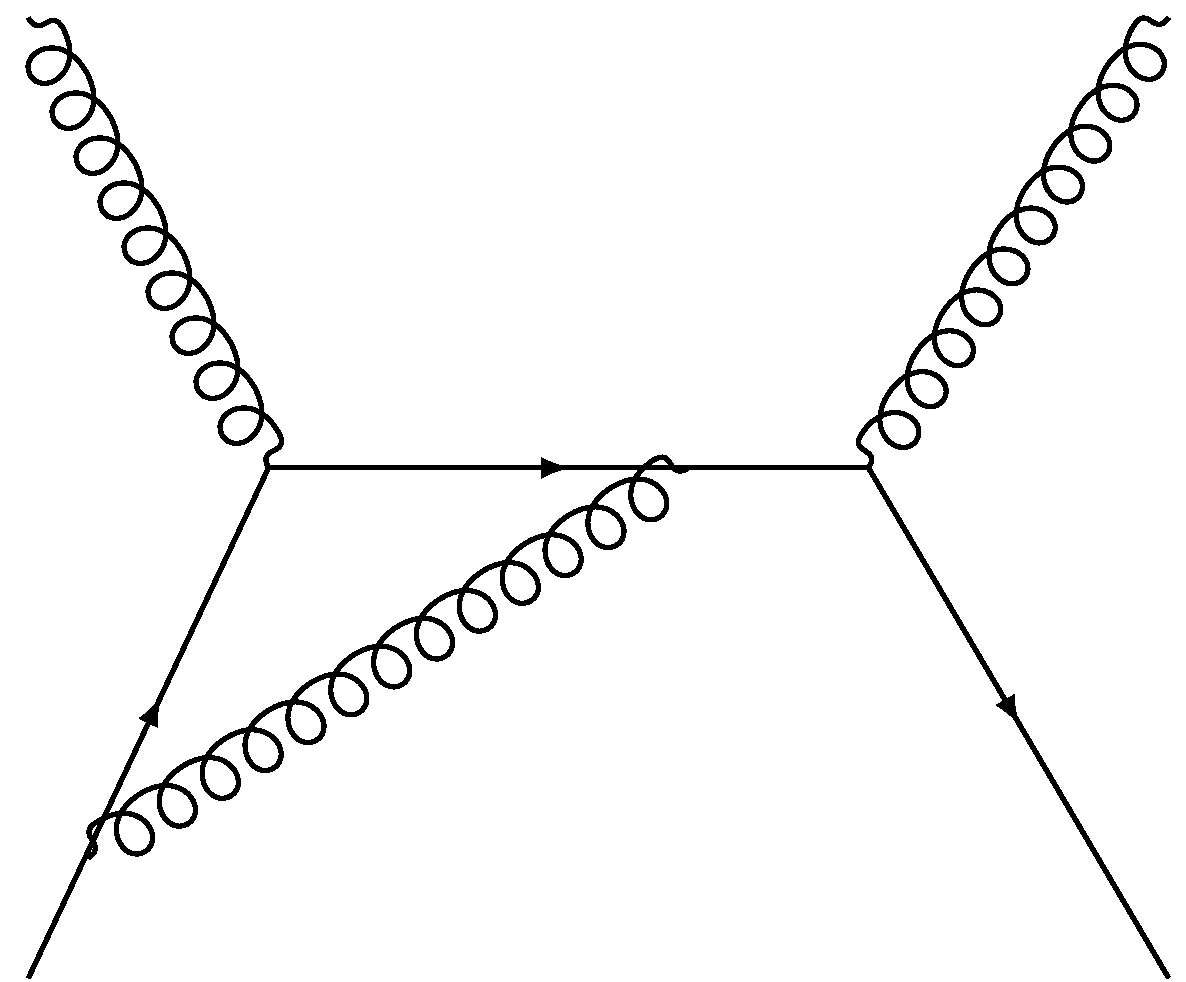
\includegraphics[scale=0.2]{Figures/An Example Diagram.pdf}
    \caption{Diagram that has no IR-divergences.}
    \label{fig:Gluon connected to propagator}
\end{figure}

The first step is to decouple $H$ from $S$. Diagrams such as \cref{fig:Gluon connected to propagator} does not generate IR-divergences. This is true to all order, i.e. a soft line can only generate an IR divergence if it is connected to an on-shell external line \cite{sterman_1993}. Thus, gluons that connect the soft and the hard part do not contribute to the IR-divergences, i.e. the soft and hard part cannot be connected directly. The physical interpretation of such a decoupling is that soft gluons correspond to large length scales, while the hard part takes place at small length scales. Therefore the soft gluons are unable to resolve the internal structure of the hard process. This fact also follows from the eikonal approximation we made in \cref{sec:wilson line properties}, where we showed that the eikonal approximation led to the concept of particles dressed with Wilson lines. This was only possible if the soft emission was connected to an on-shell external line.

The second step of the argument is to decouple the jets from each other. By definition all jets move in different directions, so lines in different jets are proportional to different momenta. We have two jets that meet at the hard interaction, but before that they cannot combine. Thus their collinear divergences will not mix with each other \cite{Sterman78}. Again, based on length scales the small momentum of the gluons in the $J_i$ cannot resolve the inner structure of the hard process. The decoupling of the jets from the soft part is more subtle, but since jets have large total momentum their substructure cannot be resolved by the soft gluons in $S$. However, close to the threshold there are energy restrictions on the gluons, leading to the large logarithmic corrections. Hence, the soft function does not completely decouple and we have to take it into account. This soft function can be constructed by taking the eikonal approximation of the partonic process, i.e. we can build it out of Wilson lines. We will come back to this procedure in the next section.

Close to the threshold we have that \cref{eq:partonic analogue to hadronic in mellin } and \cref{eq:threshold factorization Mellin} must be equal, giving the fully factorized hard function
\begin{align}\label{eq:partonic hard function ratio in mellin}
    \Me{\omega}_{ij}(N,Q,\mu,\alpha_s(\mu))=\frac{\Me{J}_{i/i}(N,Q,\epsilon)\Me{J}_{j/j}(N,Q,\epsilon)}{\tilde{f}_{i/i}(N,\mu,\epsilon)\tilde{f}_{j/j}(N,\mu,\epsilon)}H_{ij}(Q,\alpha_{s}(\mu))\Me{S}_{ij}(N,Q,\mu,\alpha_{s}(\mu))\,.
\end{align}

Since the partonic function is defined to be infrared safe, the ratio of the jet and parton distributions must cancel the collinear divergences. The ratio of distributions might seem strange and it may not be obvious at this point how to evaluate them. But we will show later how this is done using renormalization group equations. 

The next step going forward is to make use of what we know of Wilson lines in order to construct the soft function. We will do this by constructing an eikonal cross section, i.e. a cross section where the radiation is restricted to be soft. Then we will show that the soft function can be replaced from \cref{eq:partonic hard function ratio in mellin} by the eikonal cross section. The motivation behind this is to use the non-Abelian eikonal exponentiation theorem to calculate the eikonal cross section.  


































